%%%%%%%%%%%%%%%%%%%%%%%%%%%%%%%%%%%%%%%%%
% Journal Article
% LaTeX Template
% Version 1.3 (9/9/13)
%
% This template has been downloaded from:
% http://www.LaTeXTemplates.com
%
% Original author:
% Frits Wenneker (http://www.howtotex.com)
%
% License:
% CC BY-NC-SA 3.0 (http://creativecommons.org/licenses/by-nc-sa/3.0/)
%
%%%%%%%%%%%%%%%%%%%%%%%%%%%%%%%%%%%%%%%%%

%----------------------------------------------------------------------------------------
%	PACKAGES AND OTHER DOCUMENT CONFIGURATIONS
%----------------------------------------------------------------------------------------

\documentclass[twoside,fontsize=10pt]{article}
%\documentclass[oneside]{article}

\usepackage{lipsum} % Package to generate dummy text throughout this template
\usepackage{graphicx}

%\usepackage[sc]{mathpazo} % Use the Palatino font
\usepackage[T1]{fontenc} % Use 8-bit encoding that has 256 glyphs
%\linespread{1.05} % Line spacing - Palatino needs more space between lines
\usepackage{microtype} % Slightly tweak font spacing for aesthetics
\usepackage{listings}
\usepackage[hmarginratio=1:1,top=32mm,columnsep=20pt]{geometry} % Document margins
%\usepackage{multicol} % Used for the two-column layout of the document
\usepackage[hang, small,labelfont=bf,up,textfont=it,up]{caption} % Custom captions under/above floats in tables or figures
\usepackage{booktabs} % Horizontal rules in tables
\usepackage{float} % Required for tables and figures in the multi-column environment - they need to be placed in specific locations with the [H] (e.g. \begin{table}[H])
\usepackage{hyperref} % For hyperlinks in the PDF

\usepackage{lettrine} % The lettrine is the first enlarged letter at the beginning of the text
\usepackage{paralist} % Used for the compactitem environment which makes bullet points with less space between them
\usepackage{chngcntr}
\counterwithout{figure}{section}
\usepackage{abstract} % Allows abstract customization
\renewcommand{\abstractname}{}    % clear the title
\renewcommand{\absnamepos}{empty}
\renewcommand{\abstractnamefont}{\normalfont\bfseries} % Set the "Abstract" text to bold
\renewcommand{\abstracttextfont}{\normalfont\small\itshape} % Set the abstract itself to small italic text
\usepackage[super]{natbib}
\bibliographystyle{apalike}
\usepackage{titlesec} % Allows customization of titles
\renewcommand\thesection{\Roman{section}} % Roman numerals for the sections
\renewcommand\thesubsection{\Roman{subsection}} % Roman numerals for subsections
\titleformat*{\section}{\LARGE\scshape\centering}
\renewcommand{\bibsection}{\section*{\refname}}
\titleformat{\section}[block]{\LARGE\scshape\centering}{\thesection}{1em}{} % Change the look of the section titles
\titleformat{\subsection}[block]{\large\bfseries}{\thesubsection}{1em}{} % Change the look of the section titles
\titleformat{\subsubsection}[block]{\bfseries\textit}{\thesubsubsection}{0.1mm}{} % Change the look of the section titles
\usepackage[table,xcdraw]{xcolor}
\usepackage{caption}


\usepackage{fancyhdr} % Headers and footers
\pagestyle{fancy} % All pages have headers and footers
\fancyhead{} % Blank out the default header
\fancyfoot{} % Blank out the default footer
\fancyhf{}
\renewcommand{\headrulewidth}{0pt}
%\fancyhead[C]{Running title $\bullet$ November 2012 $\bullet$ Vol. XXI, No. 1} % Custom header text
\fancyfoot[RO,LE]{\thepage} % Custom footer text

%----------------------------------------------------------------------------------------
%	TITLE SECTION
%----------------------------------------------------------------------------------------

\title{\vspace{-15mm}\fontsize{18pt}{10pt}\normalfont\textbf{Everything should be linked: linking and visualising data for dynamic multilevel and multidimensional biological data interpretation.\\ \vspace{4 mm} {{\footnotesize \textit{Exploring multi-level effects of structural variations in non-coding genomic regions in cancer}}}}} % Article title

\author{
\large
\textsc{RHWE (Robin) van der Weide}\thanks{Supervisor: Joep de Ligt, PhD}\\[2mm] % Your name
\normalsize   Cancer Stem cells \& Developmental biology \\ % Your institution
\normalsize  Utrecht Graduate School of Life Sciences \\ % Your institution
%\normalsize \href{mailto:john@smith.com}{john@smith.com} % Your email address
\vspace{-5mm}
}
\date{}

%----------------------------------------------------------------------------------------

\begin{document}

\maketitle % Insert title

\thispagestyle{fancy} % All pages have headers and footers

%----------------------------------------------------------------------------------------
%	ABSTRACT
%----------------------------------------------------------------------------------------
\newpage
\mbox{   }
\newpage
\renewcommand{\abstractname}{\begin{center}
Summary of the research
\end{center}}    % clear the title
\begin{abstract}
\noindent With the increase in popularity and cost-effectiveness of various omics-approaches, more and more data is becoming available to researchers of different fields. The complexity of integrating and analysing information of these approaches increases with every added omics-layer and/or other dimension (e.g. time-series, treatments). The current tools and frameworks for these approaches have two major limitations in their design: scalability and generality (i.e. the possibility to add of more levels and/or dimensions). Moreover, there isn't an option to overview a dataset without filtering, dividing or structuring the data. These limitations restrict the integration of complex dataset, needed to truly understand biology.
\medskip

\noindent Enter the Semantic Web and its Resource Description Framework (RDF). A simple and flexible framework for describing anything about anything. An example of such a RDF-instance (a triple) is "BRAF1 has the molecular function of binding calcium ion", which has these three parts: a subject (BRAF1), a predicate (molecular function) and an object (binding calcium ion). Another Triple can then say something about the phosphorylated protein levels of this gene in a sample. Connecting these two Triples would enable a researcher to find a possible pattern in the data (i.e. a gene, responsible for calcium ion binding, has a low phosphorylation level in the investigated sample). Since every type of data can be translated to RDF, integration of large datasets of different levels and dimensions becomes possible and a lot more feasible. Both local and remote triples can be easily combined (EMBL-EBI has already launched six databases, including UniProt and Reactome), which makes analyses even more powerful. By using the SPARQL Protocol and RDF Query Language (SPARQL), retrieving and manipulating data in RDF is easily readable by both humans and computers. The SPARQL-results can subsequently be visualized as a whole, or filtered by the user. 
\medskip

\noindent Here, we propose the use of semantic web technologies and visual analytics to decrease the complexity of integrating and visualizing multi-level and -dimensional biological data. Firstly, we will create the framework needed to design the missing tools for converting the most-used NGS-formats to RDF. Next, methods and tools for visual analytics of the biological RDF-data will be created. Previously unmanageable integration-focussed analyses on the consequences of structural variation in the non-coding regions of cancer-genomes are used to showcase the proposed methods.
\end{abstract}
\medskip
\renewcommand{\abstractname}{\begin{center}
Layman's summary
\end{center}}    % clear the title
\begin{abstract}\noindent 
\lipsum[1]
\medskip
\noindent \textbf{Keywords:} structural variation, multi-level data integration, next-generation sequencing, cancer, visual analytics
\end{abstract}



%----------------------------------------------------------------------------------------
%	ARTICLE CONTENTS
%----------------------------------------------------------------------------------------
\newpage
\section*{Background, aims and approach}
\subsection*{Overall aim}
The aim of this project is to integrate and visualise multiple levels and dimensions of (NGS-based) omics-data with methods of the semantic web and, using these methods, further understand the consequences of structural variations in the non-coding regions of the genome on other biological levels, like the transcriptome and proteome. Thus, this proposal has three sub-projects, which rely heavily on each other:

\begin{enumerate}
\item \textbf{Data-integration} 
Integration of NGS-based data by using Semantic Web-methodologies to improve integrative bioinformatics in general and NGS-based multi-level and -dimensional research in particular.
\item \textbf{Visual analytics} 
Linking the Semantic-Web data to D3.js, enabling researchers to dynamically and interactively visualise RDF.
\item \textbf{Multi-level analysis} 
Multi-level and -dimensional integrative bioinformatical analysis to elucidate the consequences of genomic structural variations in non-coding regions in cancer.
\end{enumerate}
\subsection*{Scientific relevance and challenges} % inleiding: complex bio at the moment/problemen stellen (eindigen met "in this proposal, Will.. etc)
%=================================================
%=================================================
%Explain the importance of the problem or critical barrier to progress in the field that the proposed project addresses.
%Explain how the proposed project will improve scientific knowledge, technical capability, and/or clinical practice in one or more broad fields.
%Describe how the concepts, methods, technologies, treatments, services, or preventative interventions that drive this field will be changed if the proposed aims are achieved.
%=================================================
%=================================================
The amount of (public) biological data has exploded in the last years -even outpacing Moore's law- which is the result of the advances in omics-technologies, like Next-Generation Sequencing (NGS) and Mass-Spectrometry (MS), in both performance and costs. Aside from the sheer size, a second factor for the highly complex nature of current biomedical research is the addition of other dimensions, like time-series or treatments to the aforementioned omics-levels. While there are plenty of studies on single-level data analysis, both academia and industry agree that data-integration is key to understanding the complex nature of biology more thoroughly \citep{Gomez-Cabrero2014, Huttenhower2010, Searls2005, Hamid2009}. However, only a few layers and/or dimensions have been integrated per study and results are -for the most part- cherry picked, instead of data-wide. This is mainly due to the methods used in integration-studies, which are limited due to the large amounts of parsing-time (i.e. the time to convert various file/region-formats): most of them are set up in the same manner as individual level-experiments, whereafter they are combined. The limited number of truly integrative studies use computational approaches to reconstruct biological networks. While this is a valid strategy, scaling the analysis from the bacteria used by \citet{Karr2012} and \citet{Lerman2012} to multi-cellular organisms proves to be difficult. The most obvious reasons for this are the complexity of the used mathematical methods, the integration of multiple data-sources (with varying file-formats) and/or due to the use of a set-in-stone database-structure. 
\medskip

\noindent
To overcome these scaling issues, \textbf{we propose the use of the Semantic Web: the \textit{Resource Description Framework} (RDF) and its query-language \textit{SPARQL Protocol and RDF Query Language} (SPARQL)}. RDF is a general and simple framework for making statements about subjects, which is already heavily used in fields outside of biology, enabling users to integrate and search data based on semantics. Within biology, RDF is only used sparsely and mainly focussed on external data-source integration and not on own data \cite{Belleau2008,Neumann2006,Sahoo2008}. Every RDF-statement (i.e. a Triple) has three parts: a subject, a predicate and an object (e.g. \lstinline|BRAF1 :: molecular function :: calcium ion binding|). This makes it possible to link every object to another and denote the relationship between them: no additional (file)formats are needed. 

Compared to other relational database management systems, RDF is completely flexible: no database-schemas (pre-specified structures for the data, like the mySQL-method of \citet{Low2013}) are needed. Aside from the low complex, flexible and self-describing nature of the RDF-data, triples can be seen as a modular directed graph: users can combine multiple relevant RDF-sources (e.g. UniProt and Proteomics-data). Every additional RDF-source results in a more relevant and heterogeneous population of triples, making the network more complex and informative. Extracting relevant information from this "hairball" of linked objects and subjects has been a major issue and challenge since the beginning of big data, as \citet{Pavlopoulos2008} stated in 2008. SPARQL provides this ability to filter on an arbitrary number of (human-readable) expressions and can combine multiple databases to query, like the RDF-databases of EMBL-EBI \citep{Jupp2014}. 
\medskip

\noindent
When data is integrated in Semantic Web RDF-database (TripleStore) and a relevant set of subjects, predicates and/or object is extracted using SPARQL, the remaining dataset is still very large. The abstract and complex nature of this "hairball" makes it hard to formalise an analytical problem to solve. \textbf{To create interactive and dynamic visual representations of a dataset, we propose to use of the multidisciplinary theories and methods of \textit{visual analytics}}. \citet{Thomas2005} describe this field in 2005 as "\textit{Visual analytics is the science of analytical reasoning facilitated by interactive visual interfaces.}". It uses analytical methods from fields as computer science and statistics to 
perform analyses and visualisation-techniques from cognitive and design sciences, such that the data can be effectively analysed (i.e. hypotheses formed and analysed) by the user.
\medskip

\noindent
Usage case: structural variants of non-coding regions in cancer


%\cite{Gomez-Cabrero2014} geeft mooie inleiding (en over de wensen van de community)

\begin{figure}[H]
    \centering
    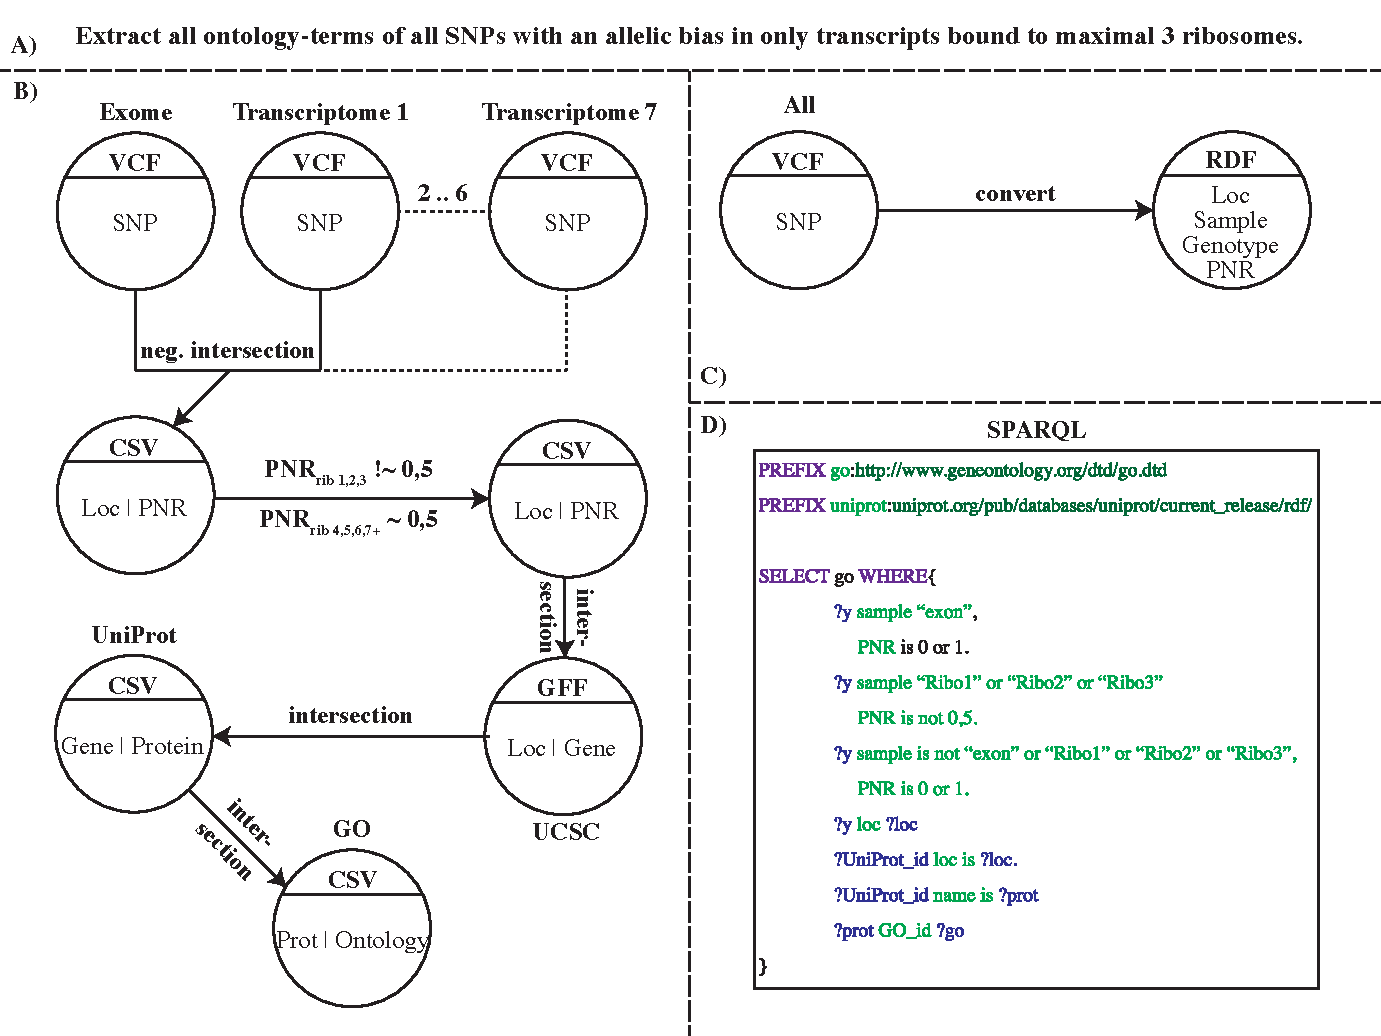
\includegraphics[width=0.75\textwidth]{DifferencesInDoingThings}
    \caption{\textbf{Differences between current integration techniques and RDF.} When a researcher has a question like \textbf{A}, he/she has to go through a series of parsing and interception steps (data juggling), like in \textbf{B}. External sources have to be fully downloaded and converted, before use. Using our proposed pipeline (shown in \textbf{C}), results in the standard conversion to RDF. Then, a question can be formulated in SPARQL (\textbf{D}), incorporating relevant outside sources, which can be easliy changed without having to juggle the data again.}
    \label{fig:awesome_image}
\end{figure}
\subsection*{Originality and innovative character} 
%=================================================
%=================================================
%Explain how the application challenges and seeks to shift current research or clinical practice paradigms.
%Describe any novel theoretical concepts, approaches or methodologies, instrumentation or interventions to be developed or used, and any advantage over existing methodologies, instrumentation, or interventions.
%Explain any refinements, improvements, or new applications of theoretical concepts, approaches or methodologies, instrumentation, or interventions.
%=================================================
%=================================================
%\cite{Sahoo2008} geeft heel veel info over BIO-RDF. Information gain through entailment reasoning is an important advantage of ontology-based data integration.

EDWINS PRESENTATIE: ONE-DIMENSIONAL DATA STILL REQUIERS OTHER DATAT TYPES - SMALL RNA-SEQ, CHIP-SEQ ETC
INTERGRATION IS VERY HARD: MET ALBERT HECK KOSTTE HET TWEE MAANDEN OM DATA TE GENEREREN EN TWEE JAAR OM TE INTEGREREN EN ANALYSEREN.

ALBERT HECK: GROOT ONDERZOEK OVER STAMCELLEN: DATA INTEGRATIE AND MINING IN AUSTRALIE... PCA VAN PROT, RNA, GEN AND METH KOMEN OVEREEN



There have already been various studies on integration of biological signals with the aid of semantic web technologies. However, the momentum is lacking: until 2014, no big databases were available in RDF-format. This meant that bioinformamtical research involving RDF had no momentum, as they could only integrate their own data, like the integration of RDF-methods in microarray analyses by \citet{Szpakowski2009} in 2009. Recently, EMBL-EBI has opened their own RDF-platfom, boasting six big data-sources (Gene Expression Atlas, ChEMBL, BioModels, Reactome, BioSamples and UniProt \cite{Jupp2014}. This was the boost of momentum needed to further incorporate RDF in biological analyses.

However, there are two main limitations of this relatively young incorporation: a standard language for denoting triples (e.g. chromosome locations) is missing and the focus lies at linking database-accessions \citep{Ruttenberg2007}. While the first limitation is also a strength (everybody can use their own dialect), a standardisation-step will enable researchers in all fields of biology to fully benefit from the integrative benefits of the Semantic Web. The second limitation is  severely restricting the use of RDF in NGS- and MS-based methods: there are no tools to convert the common formats, like the \textit{Variant Call Format} (VCF) and \textit{Sequence Alignment Format} (SAM), to triples. One of the main innovative points of our proposal is the development of methods to handle these NGS- and MS-based formats for use in the Semantic Web. This will result in a broader use of semantic web-technologies for the research community, by enabling the coupling of (own) NGS- and MS-data to existing RDF-databases.
\medskip

\noindent
added value of linked data visual analytics TOV standaard methodes
\medskip

\noindent
innovatie van cancer NC-SV
\subsection*{Methods and techniques} %M&M
%=================================================
%=================================================
%Describe the overall strategy, methodology, and analyses to be used to accomplish the specific aims of the project. Include how the data will be collected, analyzed, and interpreted as well as any resource sharing plans as appropriate.
%Discuss potential problems, alternative strategies, and benchmarks for success anticipated to achieve the aims.
%As applicable, also include the following information as part of the Research Strategy, keeping within the three sections listed above: Significance, Innovation, and Approach.
%=================================================
%=================================================
\section*{Research plan}
\subsection*{Timetable}
% Please add the following required packages to your document preamble:
% \usepackage[table,xcdraw]{xcolor}
% If you use beamer only pass "xcolor=table" option, i.e. \documentclass[xcolor=table]{beamer}
\begin{center}

\begin{table}[h]
\begin{tabular}{lllllllll}
                                                & \multicolumn{8}{c}{Semesters}                                                                                                                                                                                                                                                                                                                                                                                 \\ \cline{2-9} 
                                                & S1                                              & S2                                              & S3                                              & S4                                              & S5                                              & S6                                              & S7                                              & S8                                              \\ \hline
\textbf{Data acquisition}                       & \cellcolor[HTML]{343434}{\color[HTML]{656565} } & \cellcolor[HTML]{343434}{\color[HTML]{656565} } & \cellcolor[HTML]{343434}{\color[HTML]{656565} } & \cellcolor[HTML]{343434}{\color[HTML]{656565} } & \cellcolor[HTML]{343434}{\color[HTML]{656565} } & \cellcolor[HTML]{343434}{\color[HTML]{656565} } & \cellcolor[HTML]{343434}{\color[HTML]{656565} } & \cellcolor[HTML]{343434}{\color[HTML]{656565} } \\
\textbf{Aim 1: Data-integration}                & \cellcolor[HTML]{343434}                        & \cellcolor[HTML]{343434}                        & \cellcolor[HTML]{343434}                        &                                                 &                                                 &                                                 &                                                 &                                                 \\
\hspace*{1em} Developing omics-specific triples & \cellcolor[HTML]{656565}                        &                                                 &                                                 &                                                 &                                                 &                                                 &                                                 &                                                 \\
\hspace*{1em} Coding conversion-tools           &                                                 & \cellcolor[HTML]{656565}                        & \cellcolor[HTML]{656565}                        &                                                 &                                                 &                                                 &                                                 &                                                 \\
\hspace*{1em} Writing Best-Practices            &                                                 &                                                 & \cellcolor[HTML]{656565}                        &                                                 &                                                 &                                                 &                                                 &                                                 \\
\textbf{Aim 2: Visual analytics}                &                                                 &                                                 & \cellcolor[HTML]{343434}                        & \cellcolor[HTML]{343434}                        &                                                 &                                                 &                                                 &                                                 \\
\hspace*{1em} Coding SPARQL+D3 endpoint         &                                                 &                                                 & \cellcolor[HTML]{656565}                        &                                                 &                                                 &                                                 &                                                 &                                                 \\
\hspace*{1em} Adding visualisation-methods      &                                                 &                                                 & \cellcolor[HTML]{656565}                        & \cellcolor[HTML]{656565}                        &                                                 &                                                 &                                                 &                                                 \\
\hspace*{1em} Adding filtering and output       &                                                 &                                                 &                                                 & \cellcolor[HTML]{656565}                        &                                                 &                                                 &                                                 &                                                 \\
\textbf{Aim 3: Multi-level analysis}            &                                                 &                                                 &                                                 &                                                 & \cellcolor[HTML]{343434}{\color[HTML]{343434} } & \cellcolor[HTML]{343434}{\color[HTML]{343434} } & \cellcolor[HTML]{343434}{\color[HTML]{343434} } & \cellcolor[HTML]{343434}{\color[HTML]{343434} } \\
\hspace*{1em} Consequences of Cancer-SV's       &                                                 &                                                 &                                                 &                                                 & \cellcolor[HTML]{656565}                        & \cellcolor[HTML]{656565}                        & \cellcolor[HTML]{656565}                        & \cellcolor[HTML]{656565}                        \\
\textbf{Writing thesis}                         &                                                 &                                                 &                                                 &                                                 &                                                 &                                                 &                                                 & \cellcolor[HTML]{343434}                       
\end{tabular}
\end{table}

\end{center}
\subsection*{Collaboration}
possibles:

Horizon-groep (cancer gneomics centre)

rdf-mensen (Marco Roos, Joachim baran, japanner\&rus)
\section*{Knowledge utilisation}
stukje over implementatie van RDF: bestaande grote bronnen en mijn uitbreiding tools en vocabulair geeft RDF onderzoekers de mogelijkehid om daadwerkelijke data-integratie studies op te zetten met easy-of-install and -use. Het feit dat er al statistische paketten zijn in de statistical software enivorment of choice -R- betekend dat gebruikers alleen RDF+SPARQL hoeven te leren, maar dat onderliggende statistical analyses op the gefilterede SPARQL-queries gewoon in R kunnen worden gedaan.  

In a broader perspective: het uitrbreiden van het semantic web (door NGS-based triple stores) leidt tot een 

linked data visual analystic zijn in alle velden te grebruiken, die RDf gebruiken. Ook voor bedrijven (pharma!). Super handig!

Vrij snel te incorpporeren: de meeste dingen zijn er al

cancer NC-SV is nog weinig over bekend: mogelijke nieuwe targets voor cancer screening and or treatment: sociaal en pharma.


%\cite{Gomez-Cabrero2014} geeft wensen van de community aan

%-------------------------------------------------------
%	REFERENCE LIST
%----------------------------------------------------------------------------------------

%\begin{thebibliography}{99} % Bibliography - this is intentionally simple in this template

%\renewcommand{\refname}{\LARGE\scshape\centering References} %
%\titleformat*{\section}{\LARGE\scshape\centering}
%\titleformat{\section}[block]{\LARGE\scshape\centering}{\thesection.}{1em}{} % Change the look of the section titles
\bibliography{library}
 
%\end{thebibliography}
%
%%----------------------------------------------------------------------------------------
%
%%\end{multicols}

\end{document}
